\subsubsection{Insertion}

Figure \ref{fig:algorithm:integer:example_1} already described some of the flow of insertion, so in here will show the table if insert a negative value into the table. Insert a -2147483647 (128-0-0-1) into table, which will become like figure \ref{fig:algorithm:integer:insertion:example_1}.

\begin{figure}[h]
\centering
%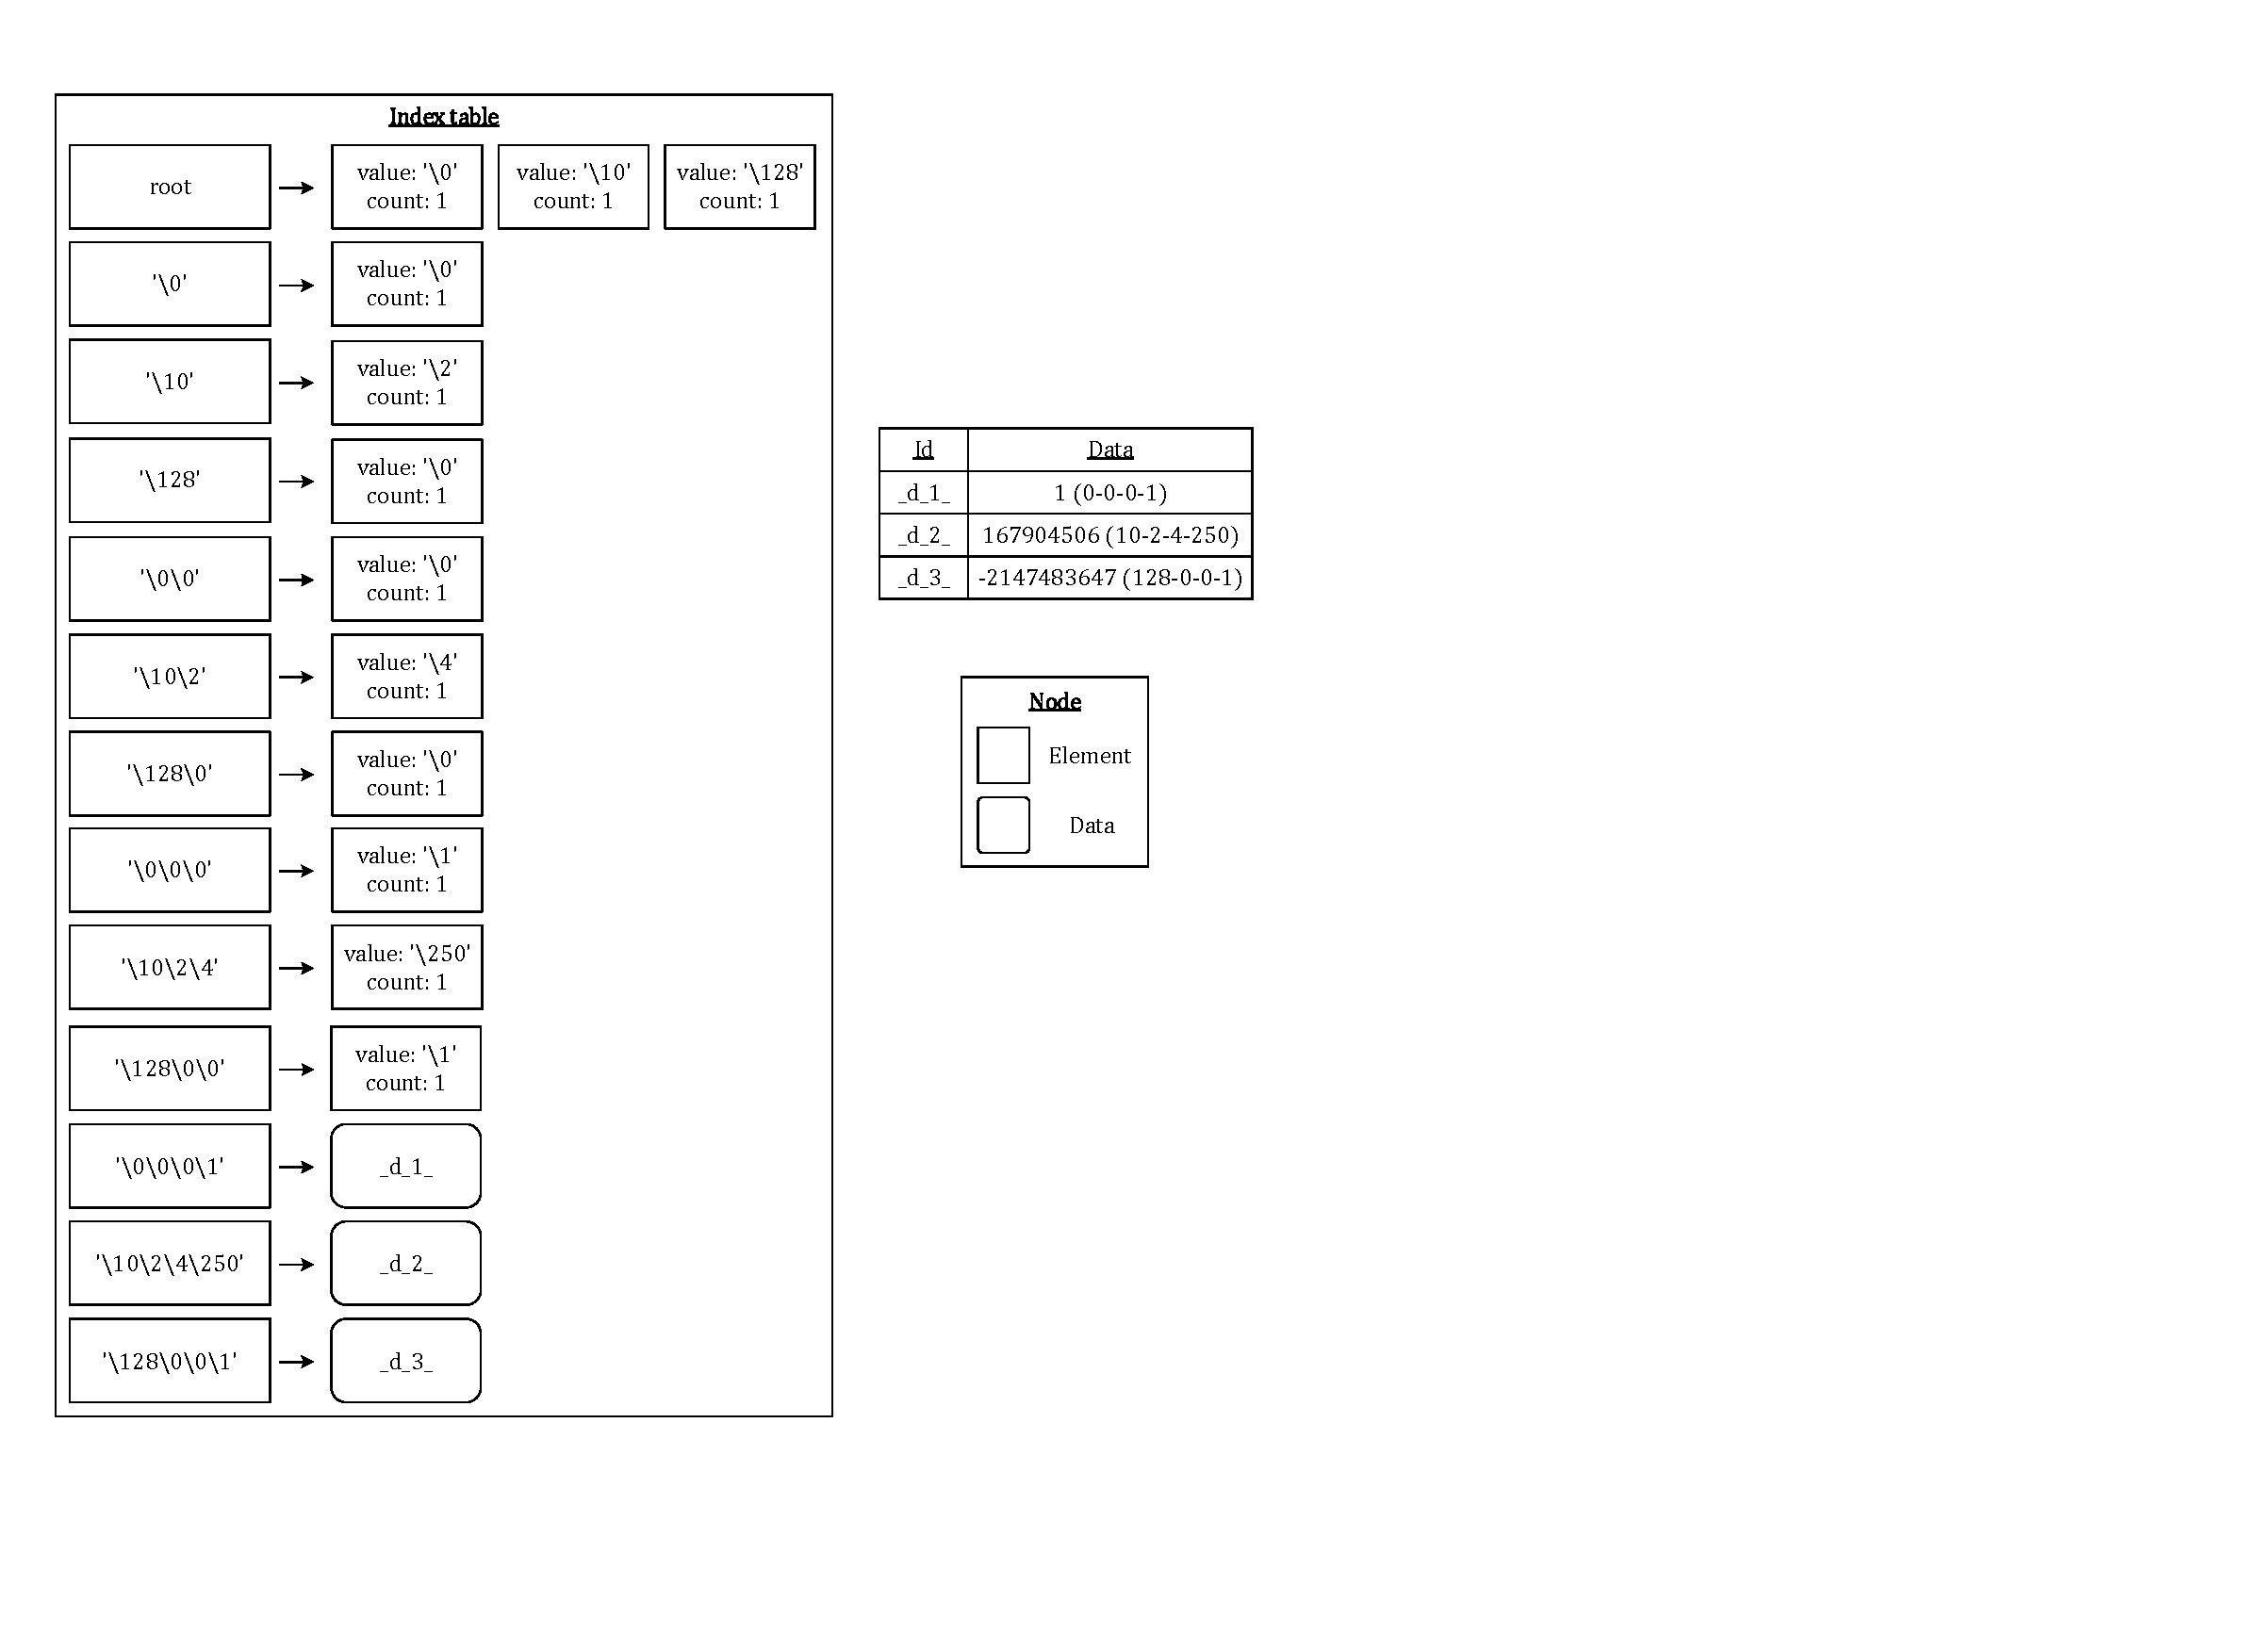
\includegraphics[scale=0.6]{./algorithm/integer/pic/insertion/example_1_v3.pdf}
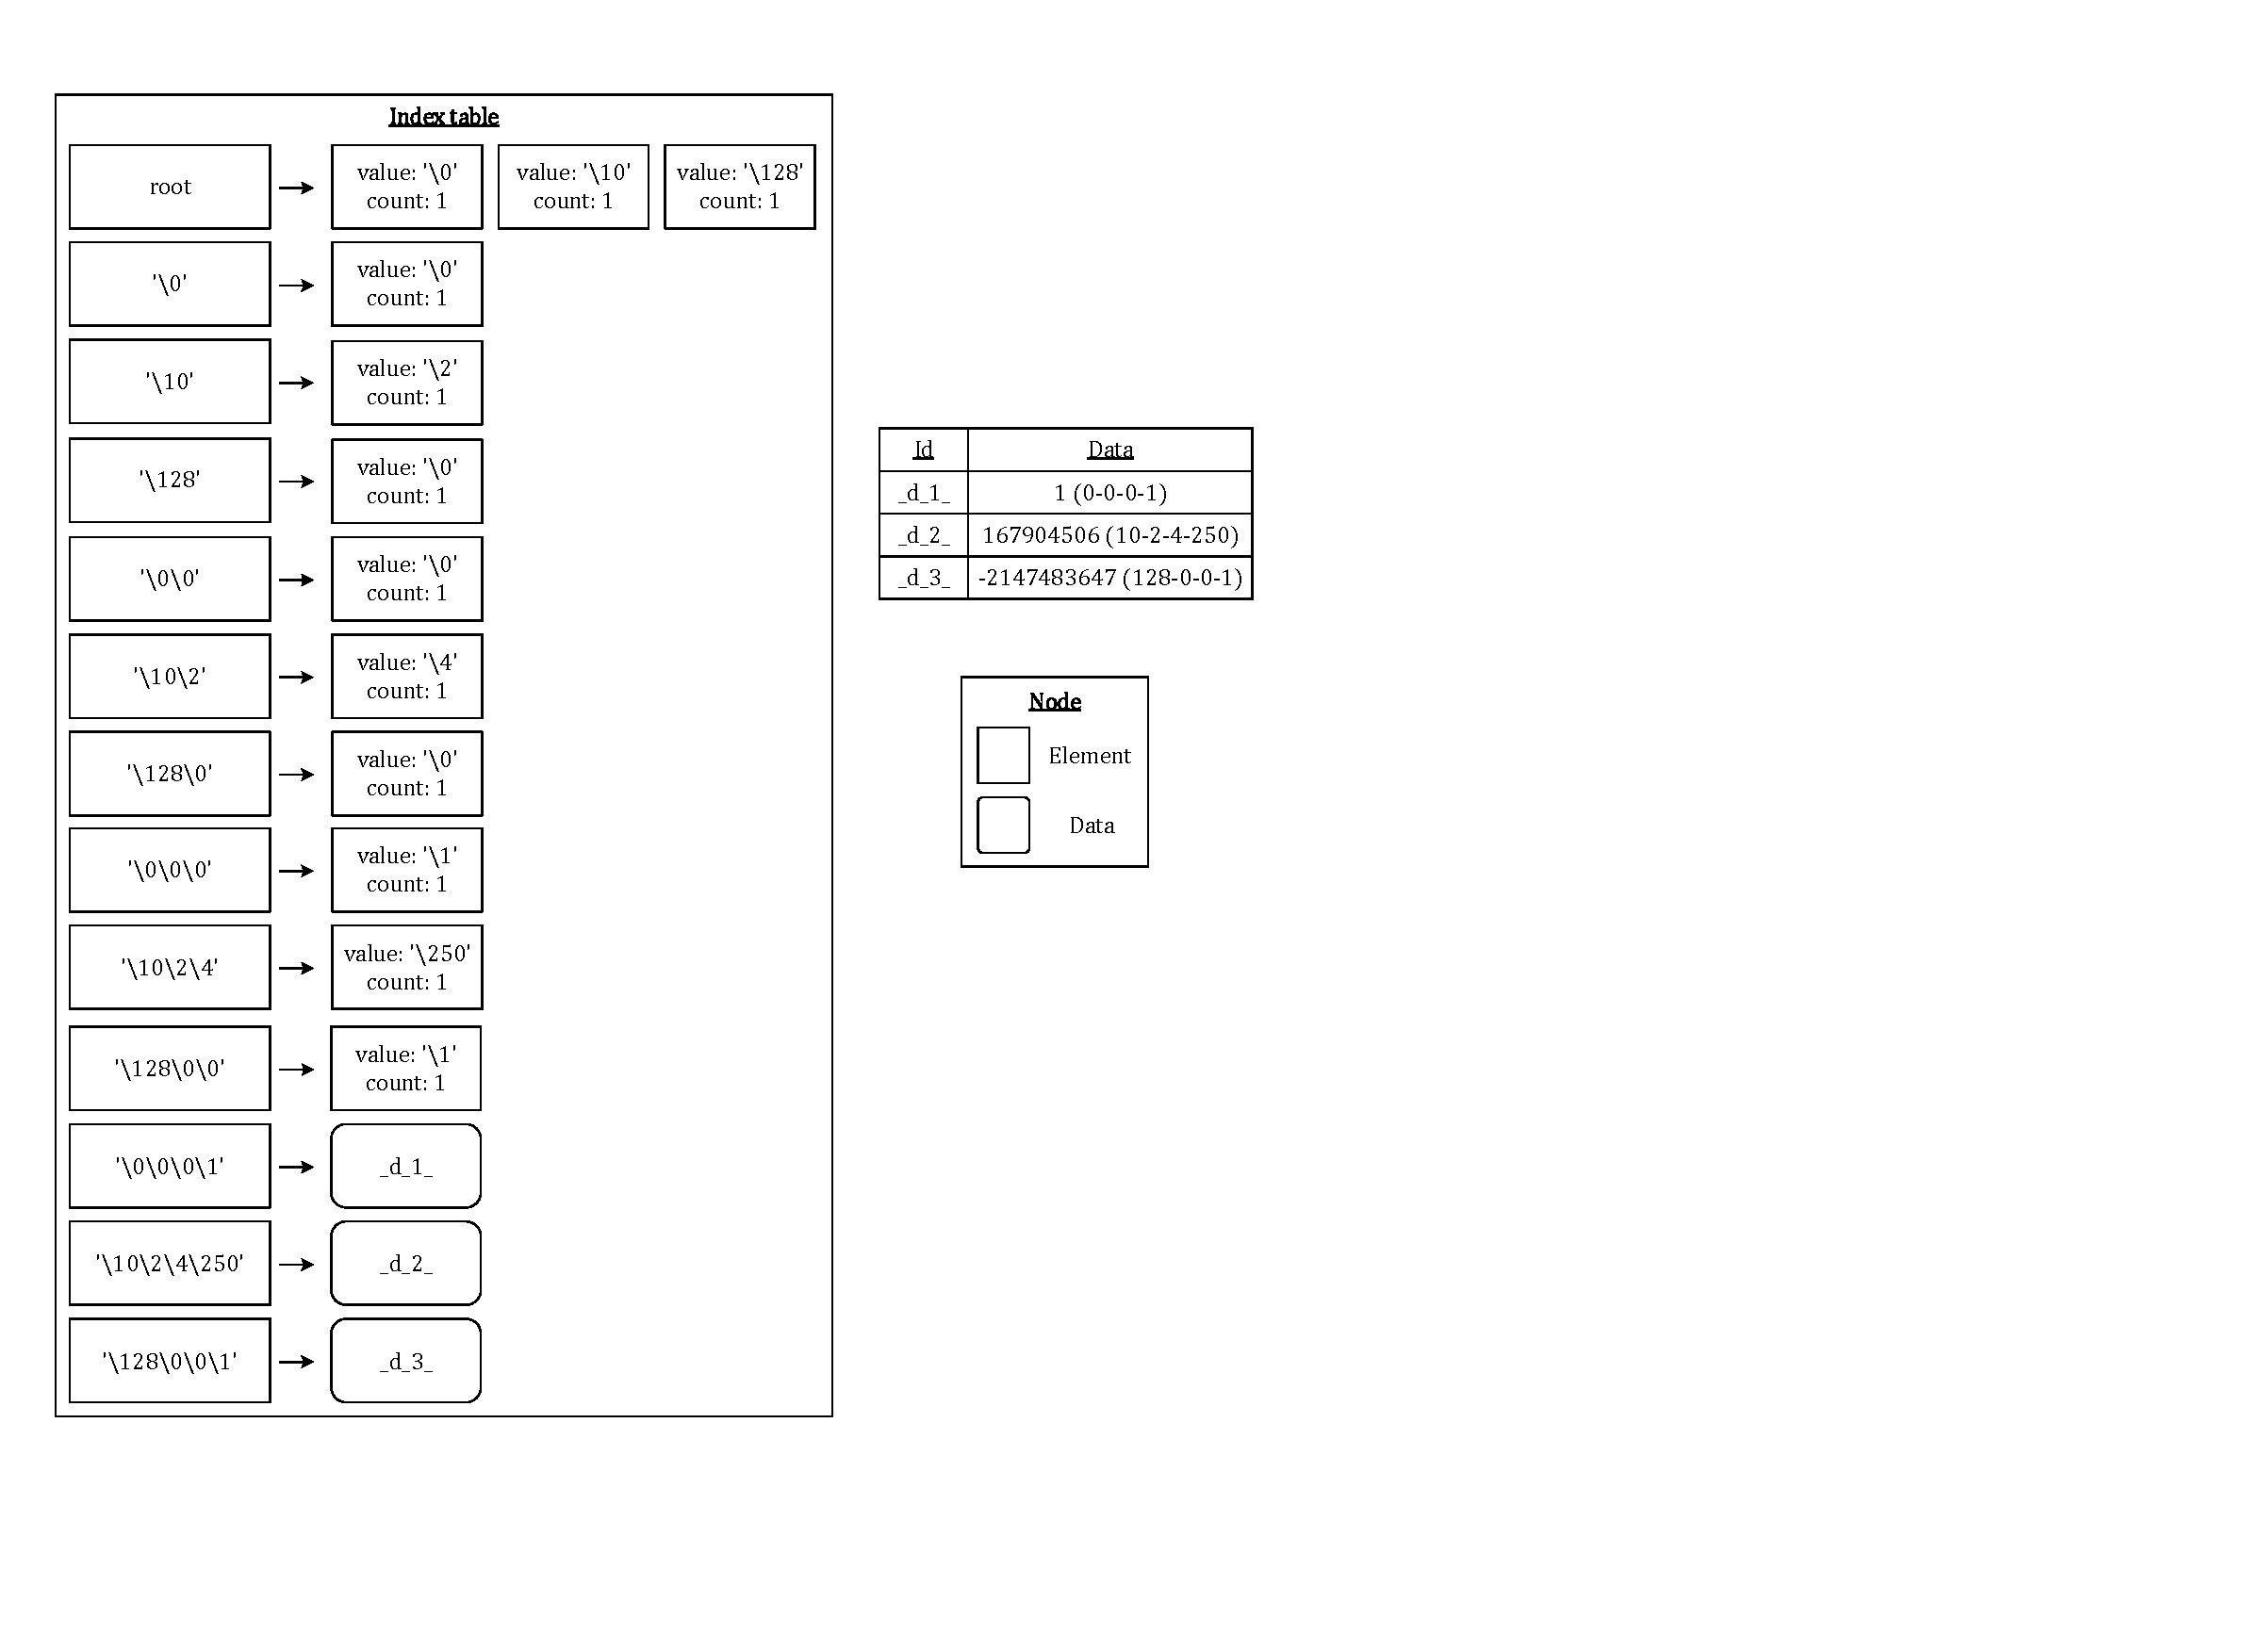
\includegraphics[width=0.8\textwidth]{./algorithm/integer/pic/insertion/example_1_v3.pdf}
\caption{The table after insert a negative value.}
\label{fig:algorithm:integer:insertion:example_1}
\end{figure}

Figure \ref{fig:algorithm:integer:insertion:example_1} shows that even a negative value will store as the same way as the positive value. And time complexity is $O(b)$.

